%!TEX root = ../../Master.tex
\section{Organization} % (fold)
\label{sec:organization}

This section will describe how the organizational structure of a hospital is and how the existing infrastructure of a hospital is including requirements for a navigation system. Hospitals have many different kinds of users, in the Administration section the focus is the administrative group; namely the regular staff, the board of directors and the region. All three groups have different traits and impacts on the hospital.

\subsection{Adminitration}

Hospitals have many different kinds of users, in this section the focus is the administrative group; namely the regular staff, the board of directors and The region. All three groups have different traits and impacts on the hospital. \\ The focus in this section is what impact indoor navigation has on the general effectiveness of the hospital and the three groups of administrative staff.\\
Hospitals can involve large and complex buildings \cite{wifi_navigation_ca} and welcomes numerous people every day. Some of those people are patients and others are the loved ones of those patients come to visit, some of whom may be entering for the first time. People who are not used to a hospital can become stressed or confused as they attempt to find an appointment, the cafeteria or the waiting rooms. As a consequence of this they ask the administrative staff for help. \cite{Frivillige_guider}

\textbf{Regular staff}: This group can be split into several subgroups containing for example the receptionist and the administrative assistant. Members of the administrative staff are often the first employees visitors will meet in a hospital, and these employees can be split into two groups in terms of how well they know the building; the new employees and the veteran employees. A new staff member may have a hard time navigating visitors or patients around in a complex facility due to a lack of knowledge of the area, whereas the veteran staff should be more knowledgeable of the facility. Even so it can still be difficult to explain a route through the facility to a visitor. Explaining it is time consuming and it will interrupt what else they might have been working on which in turn may be stressful for the staff \cite{arbejdsmiljo_ca}. If people visiting the hospital are to rely on the staff for navigation it also possesses a bottleneck as each employee can only communicate with one person at a time.

\textbf{Board of Directors and The region}: This group can be split into several subgroups containing for instance, economy and scheduling and quality, normal these groups, don't meed up with the visitors directly, but these groups are Indirectly affected by the visitors and the staff. if staff are on a tight schedule, and they run into an unforeseen workload, then their schedule will slip. this can effect appointments the staff may have. The staff will then have to work overtime, and they will then have to be paid more, effecting the economy in the hospital. A ineffective hospital will cost more money for the region, and the work will / may be of lower quality, this can prevent that the money could be used for something more useful \cite{timer_til_at_hjelpe_rundt}.

In the following we will cover which procedures are needed in order to realize a software solution for our initiating problem (\cref{sub:init}).

In a decision process the following phases will typically happen. \cite{Sjaelland}


\begin{itemize}
  \setlength{\itemsep}{1pt}
  \setlength{\parskip}{0pt}
  \setlength{\parsep}{0pt}
	\item \textbf{Idea and initiative phase} A problem is defined by the citizens, media or political organisation.
	\item \textbf{Preparing phase} The problem will be reviewed according to the health legislation.
	\item \textbf{Decision phase} The problem is presented and a committee is established. This committee will typically work with consultants to specify the requirements of the solution.
	\item \textbf{Implementation phase} The solution will be implemented. 
\end{itemize}

The highest court of the hospital is politically elected bodies: parliament, government and the minister-led ministries and the Regional Council. This was also the Regional Council on 21 September 2010 adopted Region North Jutland budget for 2011 and a budget conciliation, which included a number of structural changes and cost savings for the hospitals in the region \cite{politisk_styret_ca}. Between the decision phase and the implementation phase, the project will be announced as a public supply contract for suppliers to tender. \cite{Union2004}. Suppliers will then submit their solutions. The solution that fits the problem's requirements best, gets the contract. 



\subsection{Infrastructure}

In order to create a good navigational system for a hospital, certain factors must be considered. When deciding new features for a hospital, installation \& maintenance costs and compatibility with the existing hardware are big subjects. Therefore this section will describe existing infrastructure in hospitals and how this will affect the navigational system.

\paragraph{Wi-Fi} \label{orgwifi}

Most hospitals have good Wi-Fi coverage in the facility \cite{Millionkontrakt_giver_Ca}. A visit to \enquote{Sygehus Nord} in Aalborg revealed that multiple locations around the hospital had a sufficient amount of Wi-Fi hot spots in range, in order to be used in Location Based Services. See \cref{fig:wifi1,fig:wifi2,fig:wifi3}.

\begin{figure}
\centering
  \begin{minipage}{0.45\textwidth}
    \centering
    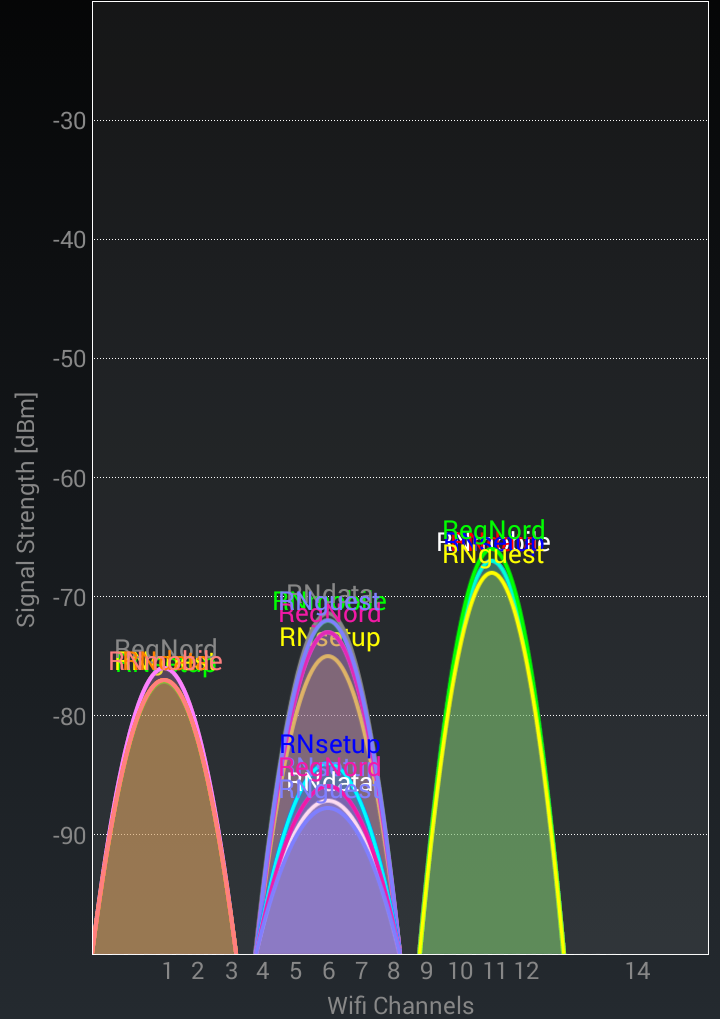
\includegraphics[width=\textwidth]{wifi_sygehus_nord1.png}
    \caption{Graph of signal strength grouped by channels. Location A} \label{fig:wifi1}
  \end{minipage}
  \hfill
  \begin{minipage}{0.45\textwidth}
    \centering
    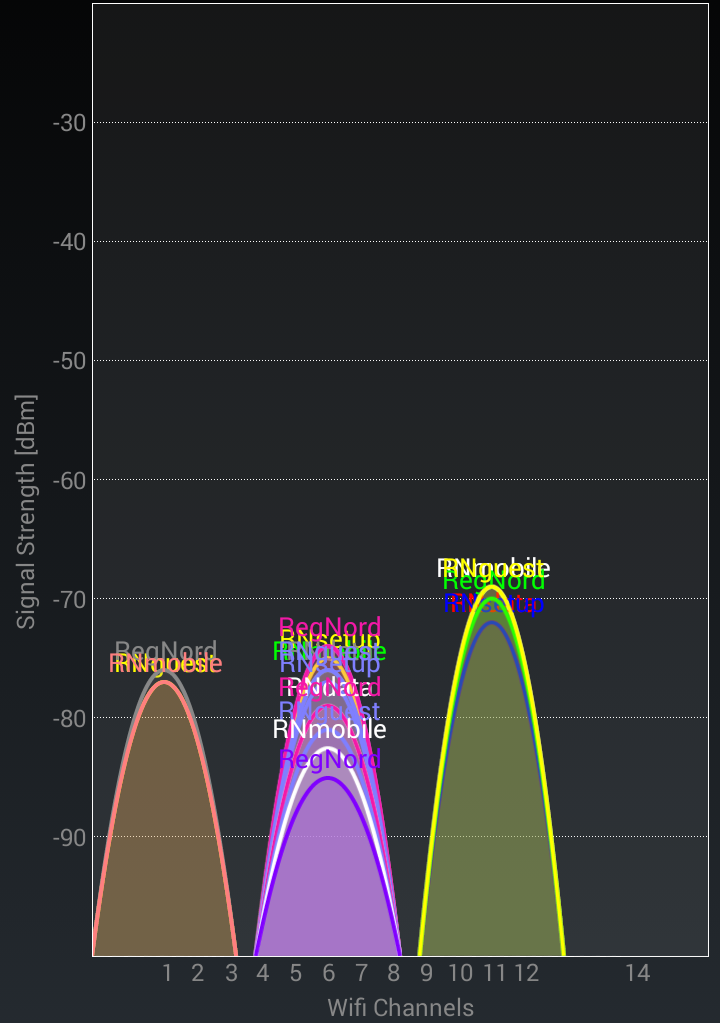
\includegraphics[width=\textwidth]{wifi_sygehus_nord2.png}
    \caption{Graph of signal strength grouped by channels. Location B} \label{fig:wifi2}
  \end{minipage}
    \begin{minipage}{0.45\textwidth}
    \centering
    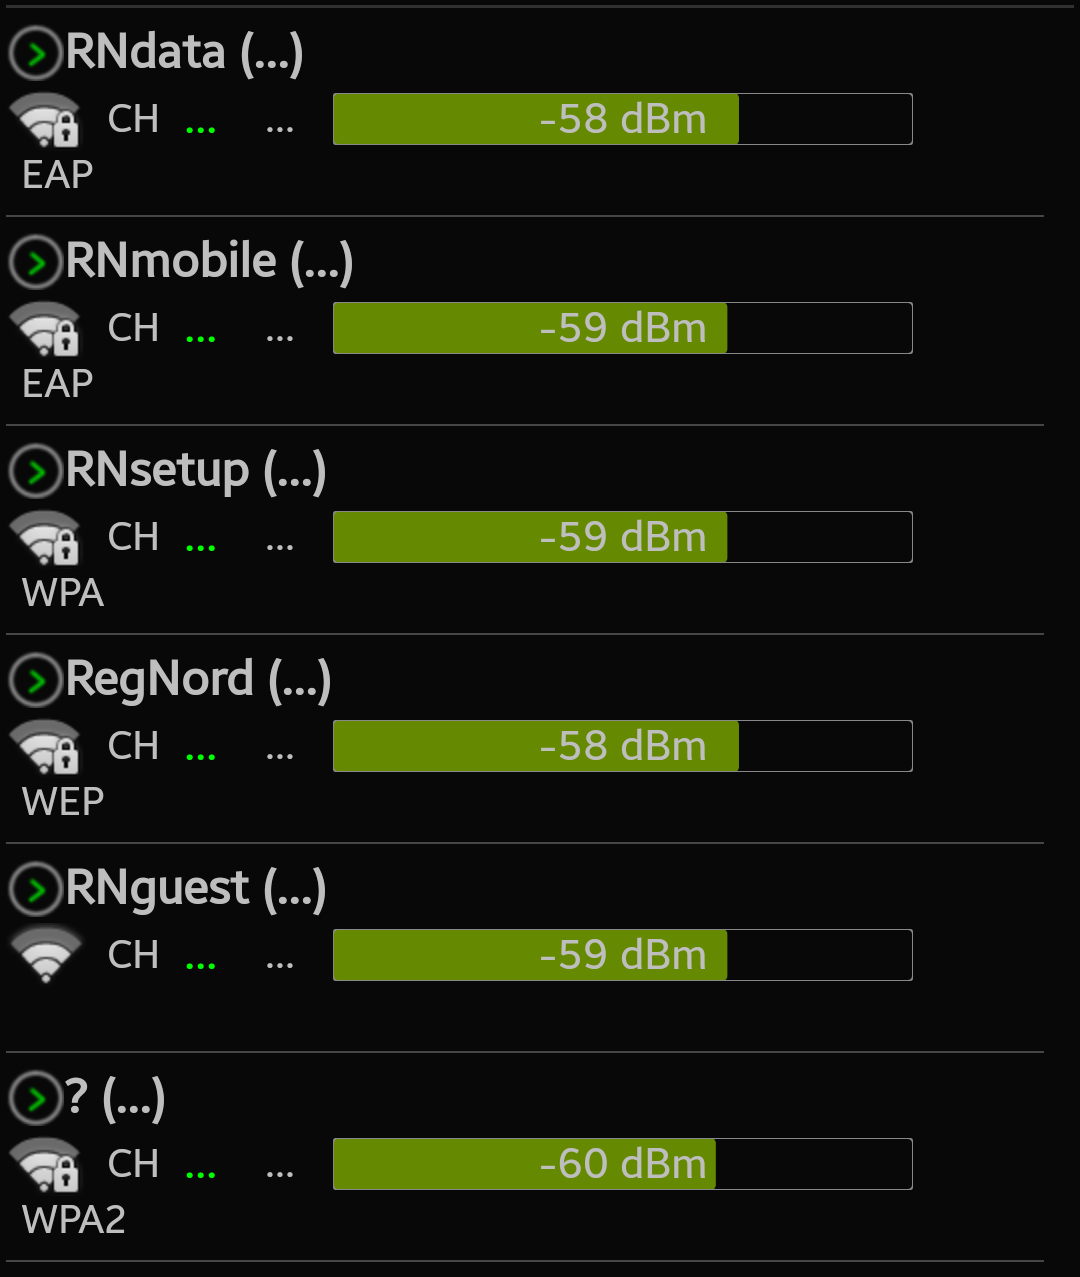
\includegraphics[width=\textwidth]{wifi_sygehus_nord3.png}
    \caption{List of WiFi networks} \label{fig:wifi3}
  \end{minipage}
  \end{figure}


\paragraph{Interference with Medical Devices}

Incidents of radio frequency interference between cellular phones, radio broadcasters, WiFi devices and medical devices have been reported. Older models of pacemakers, defibrillator and hearing aid devices were being influenced by near encounter of cellular phones causing undesirable effects which could lead to uncontrollable heartbeat. 
The problem was that radio frequency fields were interfering with medical equipment. This has however now been addressed in modern standards, meaning that interference with medical devices does not occur any more \cite{Man1998,Case}.

\paragraph{Temporary Out-of-Order Elements}

When mapping a hospital every hall building, stair, elevator etc. has to be considered. Situations may however occur in which some of the mapped elements in fact are temporarily out-of-order. This could be an elevator or a hallway being repainted. Updating the navigation system map to include the temporary elements would be a lot of effort. In a situation in which an user of the navigation system is guided through an out-of-order element, the user will most likely find their own way around this obstacle. When this happens, the user is going off-route. The navigation system must support this and act accordingly.

\paragraph{Cross-Building Support}

Some hospitals will undoubtedly have several building complexes around their cadastral. A good navigational system should work across these platforms providing one, uniform experience. This is both good for the end-user but also eases the maintenance work for the the navigational, because it can be reused across many different hospitals. If support for cross-building complexes has been laid, this could further expand to the navigation system supporting different hospitals independent of each other. The navigation system could then e.g. be installed in all the hospitals in Region Nordjylland, providing an uniform experience for end-users.

\subsection{Summary of Organization}

To round up, the extra workload that can occur when navigating in a hospital is a problem, because it is time consuming and stressful for both the regular staff and the visitors. The problem is not only affecting visitors but also the staff working at the hospital. 

Changes in a hospital can occur when the region decides to save or spend money. The infrastructure or structure in general can be modified. When these decisions are made, 3 different phases are typically executed: preparing phase, decision phase and implementation phase. When changes are to be made, installation \& maintenance costs and compatibility with the existing hardware, are big subjects.


% section organization (end)